\documentclass[12pt,a4paper]{article}

% ─── Packages ────────────────────────────────────────────────────────────────
\usepackage{amsmath, amssymb, amsthm}
\usepackage{geometry}
\usepackage{hyperref}
\usepackage{tikz}
\usepackage{pgfplots}
\pgfplotsset{compat=1.18}
\usetikzlibrary{arrows.meta, calc, positioning, shapes.geometric,
                decorations.pathreplacing, backgrounds, fit}
\usepackage{xcolor}
\usepackage{tcolorbox}
\tcbuselibrary{theorems, skins, breakable}
\usepackage{booktabs}
\usepackage{array}
\usepackage{enumitem}
\usepackage{mathrsfs}
\usepackage{fancyhdr}
\usepackage{titlesec}
\usepackage{microtype}
\usepackage{setspace}

% ─── Page Geometry ────────────────────────────────────────────────────────────
\geometry{margin=2.5cm, top=3cm, bottom=3cm}
\setlength{\headheight}{14pt}
\setstretch{1.15}

% ─── Colours ──────────────────────────────────────────────────────────────────
\definecolor{axiomblue}{RGB}{30, 80, 160}
\definecolor{defgreen}{RGB}{20, 130, 80}
\definecolor{thmred}{RGB}{160, 30, 40}
\definecolor{notegray}{RGB}{90, 90, 90}
\definecolor{shadeblue}{RGB}{230, 240, 255}
\definecolor{shadegreen}{RGB}{225, 248, 235}
\definecolor{shadered}{RGB}{255, 235, 235}
\definecolor{shadeyellow}{RGB}{255, 252, 220}
\definecolor{purpleshade}{RGB}{240, 230, 255}
\definecolor{purpledark}{RGB}{100, 30, 160}

% ─── Header / Footer ─────────────────────────────────────────────────────────
\pagestyle{fancy}
\fancyhf{}
\fancyhead[L]{\small\textit{Linear Algebra}}
\fancyhead[R]{\small\textit{Subspaces, Span \& Linear Systems}}
\fancyfoot[C]{\thepage}
\renewcommand{\headrulewidth}{0.4pt}

% ─── Section Formatting ───────────────────────────────────────────────────────
\titleformat{\section}{\large\bfseries\color{axiomblue}}{\thesection}{1em}{}[\titlerule]
\titleformat{\subsection}{\normalsize\bfseries\color{defgreen}}{\thesubsection}{1em}{}
\titleformat{\subsubsection}{\normalsize\bfseries\color{notegray}}{\thesubsubsection}{1em}{}

% ─── Theorem Environments ─────────────────────────────────────────────────────
\tcbset{
  defstyle/.style={
    enhanced, colback=shadegreen, colframe=defgreen,
    fonttitle=\bfseries, breakable
  },
  thmstyle/.style={
    enhanced, colback=shadered, colframe=thmred,
    fonttitle=\bfseries, breakable
  },
  axiomstyle/.style={
    enhanced, colback=shadeblue, colframe=axiomblue,
    fonttitle=\bfseries, breakable
  },
  notestyle/.style={
    enhanced, colback=shadeyellow, colframe=orange!70!black,
    fonttitle=\bfseries, breakable
  },
  propstyle/.style={
    enhanced, colback=purpleshade, colframe=purpledark,
    fonttitle=\bfseries, breakable
  }
}

\newtcbtheorem[number within=section]{definition}{Definition}{defstyle}{def}
\newtcbtheorem[number within=section]{theorem}{Theorem}{thmstyle}{thm}
\newtcbtheorem[number within=section]{proposition}{Proposition}{propstyle}{prop}
\newtcbtheorem[number within=section]{remark}{Remark}{notestyle}{rem}
\newtcbtheorem[number within=section]{example}{Example}{notestyle}{ex}

% ─── Math Operators ───────────────────────────────────────────────────────────
\newcommand{\R}{\mathbb{R}}
\newcommand{\vv}[1]{\mathbf{#1}}
\newcommand{\vzero}{\mathbf{0}}
\newcommand{\norm}[1]{\left\lVert #1 \right\rVert}
\DeclareMathOperator{\Span}{Span}
\DeclareMathOperator{\nullspace}{N}

\renewcommand{\qedsymbol}{$\blacksquare$}

% ══════════════════════════════════════════════════════════════════════════════
\begin{document}
% ══════════════════════════════════════════════════════════════════════════════

% ─── Title Page ──────────────────────────────────────────────────────────────
\begin{titlepage}
  \centering
  \vspace*{3cm}
  {\Huge\bfseries\color{axiomblue} Linear Algebra}\\[0.8em]
  {\huge\bfseries Subspaces, Span \& Linear Systems}\\[2em]
  \rule{0.6\linewidth}{1.5pt}\\[2em]
  {\large\itshape A Comprehensive Mathematical Treatment}\\[1em]
  {\normalsize Covering subspace theory, null spaces of matrices,\\
  linear combinations, spanning sets, and the\\
  general solution structure of linear systems.}\\[4em]
  % Pure TikZ illustration – subspace S inside V
  \begin{tikzpicture}[scale=1.1]
    % outer ellipse = V
    \draw[axiomblue, line width=2pt, fill=shadeblue!60]
      (0,0) ellipse (4.5cm and 2.8cm);
    \node[axiomblue, font=\bfseries] at (3.2, 2.1) {$V$};
    % inner ellipse = S
    \draw[defgreen, line width=1.8pt, fill=shadegreen!80]
      (-0.4,0) ellipse (2.4cm and 1.5cm);
    \node[defgreen, font=\bfseries] at (1.4, 1.2) {$S$};
    % zero vector dot
    \fill[thmred] (-0.4,0) circle(3.5pt)
      node[below=4pt, thmred, font=\small$\bfseries$] {$\vzero$};
    % a vector in S
    \draw[-{Latex[length=7pt]}, purpledark, line width=1.5pt]
      (-0.4,0) -- (0.9,0.9) node[right=2pt, font=\small]{$\vv{x}$};
    % scalar multiple stays in S
    \draw[-{Latex[length=7pt]}, defgreen, line width=1.5pt]
      (-0.4,0) -- (-1.9,-0.8) node[left=2pt, font=\small]{$\alpha\vv{x}$};
    % sum stays in S
    \draw[-{Latex[length=7pt]}, axiomblue, line width=1.5pt]
      (-0.4,0) -- (-0.1,1.1) node[above=2pt, font=\small]{$\vv{x}{+}\vv{y}$};
    % a vector outside S but in V
    \draw[-{Latex[length=7pt]}, thmred!70, line width=1.2pt, dashed]
      (0,0) -- (3.4,1.2) node[right=2pt, font=\small, thmred]{$\vv{w}\!\notin\!S$};
  \end{tikzpicture}\\[2em]
  \vfill
  {\small\color{notegray}\today}
\end{titlepage}

% ─── Table of Contents ───────────────────────────────────────────────────────
\tableofcontents
\newpage

% ══════════════════════════════════════════════════════════════════════════════
\section{Introduction}
% ══════════════════════════════════════════════════════════════════════════════

Having established the abstract notion of a vector space in the previous chapter,
we now study the \emph{internal structure} of vector spaces.  The central objects
are \textbf{subspaces} — subsets that are themselves vector spaces under the
inherited operations — together with the related notions of \textbf{span},
\textbf{linear combinations}, and \textbf{spanning sets}.

The chapter concludes by applying these ideas to the study of linear systems
$A\vv{x} = \vv{b}$, revealing that the complete solution set has a clean
geometric structure built from a particular solution and the null space of $A$.

% ══════════════════════════════════════════════════════════════════════════════
\section{Subspaces}
% ══════════════════════════════════════════════════════════════════════════════

\subsection{Definition and Closure Properties}

\begin{definition}{Subspace}{subspace}
  Let $V$ be a vector space and let $S$ be a \emph{nonempty} subset of $V$.
  $S$ is called a \textbf{subspace} of $V$ if it satisfies both of the following
  \emph{closure conditions}:
  \begin{enumerate}[label=(\roman*), leftmargin=2.5em]
    \item \textbf{Closed under scalar multiplication:}
          $\alpha\vv{x} \in S$ whenever $\vv{x} \in S$, for every scalar
          $\alpha \in \R$.
    \item \textbf{Closed under addition:}
          $\vv{x} + \vv{y} \in S$ whenever $\vv{x}, \vv{y} \in S$.
  \end{enumerate}
\end{definition}

\noindent
Condition (i) ensures that stretching or reflecting any vector in $S$ keeps the
result inside $S$.  Condition (ii) ensures that forming the sum of any two vectors
in $S$ never ``escapes'' $S$.  Together, they say that arithmetic with elements of
$S$ — using the operations of $V$ — always produces elements of $S$.

\begin{remark}{Every subspace is itself a vector space}{ssvs}
  Let $S$ be a subspace of $V$.  Using the operations of $V$ restricted to $S$,
  the system $(S, +, \cdot)$ satisfies all eight vector space axioms:
  \begin{itemize}[leftmargin=2em]
    \item \textbf{A1, A2, A5--A8} hold for any elements of $V$, so in particular
          for elements of $S$.
    \item \textbf{A3} (existence of $\vzero$): By condition (i),
          $0 \cdot \vv{x} = \vzero \in S$ for any $\vv{x} \in S$
          (Theorem 3.1.1(i)).
    \item \textbf{A4} (additive inverse): By condition (i),
          $(-1)\vv{x} = -\vv{x} \in S$ for any $\vv{x} \in S$
          (Theorem 3.1.1(iii)).
  \end{itemize}
  Hence $S$ is a vector space in its own right.
\end{remark}

\subsection{Trivial and Proper Subspaces}

\begin{remark}{Trivial subspaces}{trivial}
  For any vector space $V$:
  \begin{itemize}[leftmargin=2em]
    \item The \textbf{zero subspace} $\{\vzero\}$ is a subspace of $V$.
          It is the smallest possible subspace.
    \item $V$ itself is a subspace of $V$.
          It is the largest possible subspace.
  \end{itemize}
  All other subspaces are called \textbf{proper subspaces} of $V$.
\end{remark}

\begin{remark}{Checking nonemptiness via $\vzero$}{nonempty}
  Every subspace must contain the zero vector, since condition (i) with
  $\alpha = 0$ gives $\vzero = 0\cdot\vv{x} \in S$.  Therefore, the most
  efficient way to verify that a candidate subset $S$ is nonempty is to
  check that $\vzero \in S$.
\end{remark}

\subsection{Geometric Interpretation in \texorpdfstring{$\R^2$}{R2} and
\texorpdfstring{$\R^3$}{R3}}

\noindent
In $\R^2$, the subspaces are exactly: $\{\vzero\}$, every line through the
origin, and $\R^2$ itself.  In $\R^3$, the proper subspaces are every
line through the origin and every plane through the origin.

\begin{center}
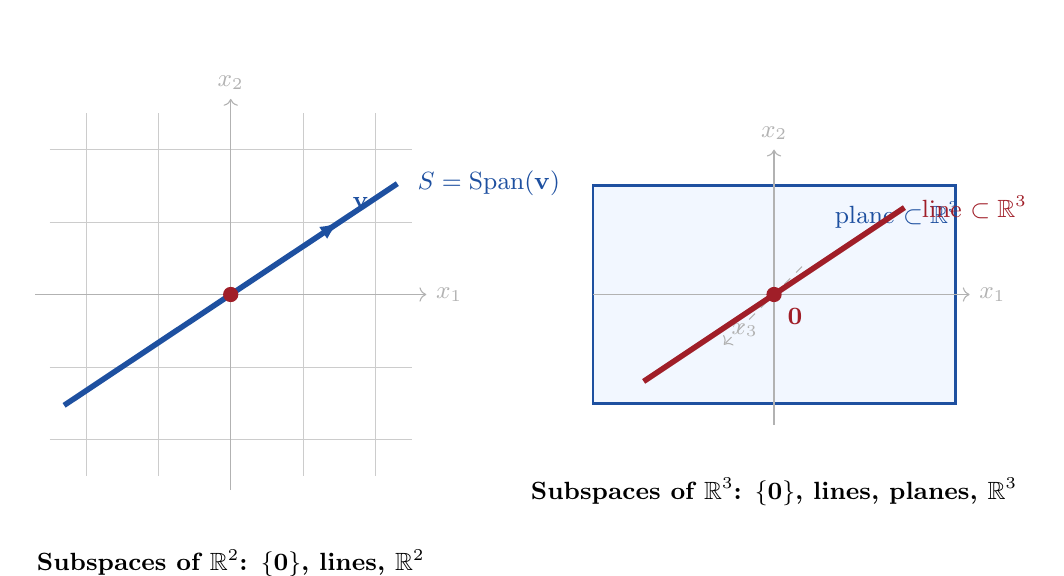
\begin{tikzpicture}[scale=0.92]
  %--- R^2 subspaces ---------------------------------------------------------
  \begin{scope}
    \draw[gray!40, very thin] (-2.5,-2.5) grid (2.5,2.5);
    \draw[->, gray!60] (-2.7,0) -- (2.7,0) node[right]{\small$x_1$};
    \draw[->, gray!60] (0,-2.7) -- (0,2.7) node[above]{\small$x_2$};
    % a subspace line
    \draw[axiomblue, line width=2pt] (-2.3,-1.53) -- (2.3,1.53)
      node[right=3pt, axiomblue, font=\small]{$S = \Span(\vv{v})$};
    \draw[-{Latex[length=7pt]}, axiomblue, line width=1.5pt]
      (0,0) -- (1.5,1) node[above right=1pt, font=\small]{$\vv{v}$};
    \fill[thmred] (0,0) circle(3pt);
    \node[below=18pt, font=\small\bfseries] at (0,-2.7)
      {Subspaces of $\R^2$: $\{\vzero\}$, lines, $\R^2$};
  \end{scope}
  %--- R^3 subspaces ---------------------------------------------------------
  \begin{scope}[xshift=7.5cm]
    % plane through origin
    \fill[shadeblue!70, opacity=0.7]
      (-2.5,-1.5) -- (2.5,-1.5) -- (2.5,1.5) -- (-2.5,1.5) -- cycle;
    \draw[axiomblue, line width=1pt]
      (-2.5,-1.5) -- (2.5,-1.5) -- (2.5,1.5) -- (-2.5,1.5) -- cycle;
    \node[axiomblue, font=\small] at (1.7,1.1){plane $\subset\R^3$};
    % axes
    \draw[->, gray!60] (-2.5,0,0) -- (2.7,0,0)
      node[right]{\small$x_1$};
    \draw[->, gray!60] (0,-1.8,0) -- (0,2.0,0)
      node[above]{\small$x_2$};
    \draw[->, gray!60,dashed] (0,0,-1) -- (0,0,1.8)
      node[above right=-1pt]{\small$x_3$};
    % a line subspace
    \draw[thmred, line width=2pt] (-1.8,-1.2) -- (1.8,1.2)
      node[right=2pt, font=\small, thmred]{line $\subset\R^3$};
    \fill[thmred] (0,0) circle(3pt)
      node[below right=2pt,font=\small]{$\vzero$};
    \node[below=0pt, font=\small\bfseries] at (0,-2.4)
      {Subspaces of $\R^3$: $\{\vzero\}$, lines, planes, $\R^3$};
  \end{scope}
\end{tikzpicture}
\end{center}

\subsection{How to Verify a Subspace}

\noindent
To show that a nonempty subset $S \subseteq V$ is a subspace, we verify
exactly three things in order:

\begin{center}
\begin{tikzpicture}[
  node distance=0.4cm and 1.8cm,
  step/.style={draw=axiomblue, fill=shadeblue, rounded corners=5pt,
               minimum width=3.6cm, minimum height=1.1cm, align=center,
               font=\small},
  arr/.style={-{Latex[length=6pt]}, axiomblue, thick}
]
  \node[step] (s0) {\textbf{Step 1}\\Show $\vzero \in S$};
  \node[step, right=of s0] (s1) {\textbf{Step 2}\\Show $\alpha\vv{x}\in S$\\for all $\vv{x}\in S,\,\alpha\in\R$};
  \node[step, right=of s1] (s2) {\textbf{Step 3}\\Show $\vv{x}+\vv{y}\in S$\\for all $\vv{x},\vv{y}\in S$};
  \node[draw=defgreen, fill=shadegreen, rounded corners=5pt,
        minimum width=2.5cm, minimum height=1.1cm, align=center,
        font=\small\bfseries, right=of s2] (s3) {$S$ is a\\subspace};
  \draw[arr] (s0) -- (s1);
  \draw[arr] (s1) -- (s2);
  \draw[arr] (s2) -- (s3);
\end{tikzpicture}
\end{center}

% ══════════════════════════════════════════════════════════════════════════════
\section{The Null Space of a Matrix}
% ══════════════════════════════════════════════════════════════════════════════

\subsection{Definition}

\begin{definition}{Null Space}{nullspace}
  Let $A$ be an $m \times n$ matrix.  The \textbf{null space} of $A$, denoted
  $N(A)$, is the set of all solutions to the homogeneous linear system
  $A\vv{x} = \vzero$:
  \[
    N(A) \;=\; \bigl\{\, \vv{x} \in \R^n \;\big|\; A\vv{x} = \vzero \bigr\}.
  \]
\end{definition}

\subsection{Proof That \texorpdfstring{$N(A)$}{N(A)} Is a Subspace of
\texorpdfstring{$\R^n$}{Rn}}

\begin{proposition}{$N(A)$ is a subspace of $\R^n$}{nullsub}
  For any $m\times n$ matrix $A$, the null space $N(A)$ is a subspace of $\R^n$.
\end{proposition}

\begin{proof}
We verify the three conditions.

\medskip
\textbf{Nonemptiness.}\quad
$A\vzero = \vzero$, so $\vzero \in N(A)$.

\medskip
\textbf{Closed under scalar multiplication.}\quad
Let $\vv{x} \in N(A)$ and $\alpha \in \R$.  Then:
\[
  A(\alpha\vv{x}) \;=\; \alpha A\vv{x} \;=\; \alpha\vzero \;=\; \vzero,
\]
so $\alpha\vv{x} \in N(A)$.

\medskip
\textbf{Closed under addition.}\quad
Let $\vv{x}, \vv{y} \in N(A)$.  Then:
\[
  A(\vv{x} + \vv{y}) \;=\; A\vv{x} + A\vv{y} \;=\; \vzero + \vzero \;=\; \vzero,
\]
so $\vv{x} + \vv{y} \in N(A)$.

\medskip
All three conditions hold; therefore $N(A)$ is a subspace of $\R^n$.
\end{proof}

\subsection{Worked Example}

\begin{example}{Computing $N(A)$ for a $2\times 4$ matrix}{nullex}
  Let
  \[
    A = \begin{pmatrix} 1 & 2 & -1 & 1 \\ 2 & 4 & -1 & 3 \end{pmatrix}.
  \]
  Row-reducing the augmented matrix $[A \mid \vzero]$:
  \[
    \begin{pmatrix}
      1 & 2 & -1 & 1 & 0 \\
      2 & 4 & -1 & 3 & 0
    \end{pmatrix}
    \;\xrightarrow{R_2 - 2R_1}\;
    \begin{pmatrix}
      1 & 2 & -1 & 1 & 0 \\
      0 & 0 &  1 & 1 & 0
    \end{pmatrix}
    \;\xrightarrow{R_1 + R_2}\;
    \begin{pmatrix}
      1 & 2 & 0 & 2 & 0 \\
      0 & 0 & 1 & 1 & 0
    \end{pmatrix}.
  \]
  Setting free variables $x_2 = s,\; x_4 = t$ gives:
  \[
    x_1 = -2s - 2t, \quad x_3 = -t.
  \]
  Therefore the general solution is:
  \[
    \vv{x}
    = s\begin{pmatrix}-2\\1\\0\\0\end{pmatrix}
    + t\begin{pmatrix}-2\\0\\-1\\1\end{pmatrix},
    \quad s, t \in \R,
  \]
  and the null space is
  \[
    N(A) = \Span\!\left(
      \begin{pmatrix}-2\\1\\0\\0\end{pmatrix},\;
      \begin{pmatrix}-2\\0\\-1\\1\end{pmatrix}
    \right).
  \]
\end{example}

\subsection{Geometric Picture of the Null Space}

\begin{center}
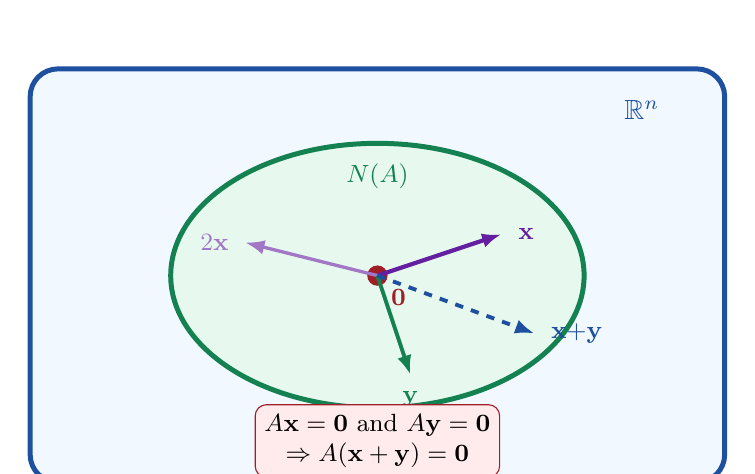
\begin{tikzpicture}[scale=1.05]
  % R^n outer box
  \draw[axiomblue, line width=1.8pt, rounded corners=10pt, fill=shadeblue!50]
    (-4.2,-2.5) rectangle (4.2,2.5);
  \node[axiomblue, font=\bfseries] at (3.2, 2.0) {$\R^n$};
  % N(A) ellipse
  \draw[defgreen, line width=1.8pt, fill=shadegreen!80]
    (0,0) ellipse (2.5cm and 1.6cm);
  \node[defgreen, font=\bfseries\small] at (0,1.2) {$N(A)$};
  % zero
  \fill[thmred] (0,0) circle(3.5pt)
    node[below right=2pt, font=\small, thmred]{$\vzero$};
  % vectors in null space
  \draw[-{Latex[length=7pt]}, purpledark, line width=1.5pt]
    (0,0) -- (1.5,0.5) node[right=2pt, font=\small]{$\vv{x}$};
  \draw[-{Latex[length=7pt]}, purpledark!60, line width=1.2pt]
    (0,0) -- (-1.6,0.4) node[left=2pt, font=\small]{$2\vv{x}$};
  \draw[-{Latex[length=7pt]}, defgreen, line width=1.4pt]
    (0,0) -- (0.4,-1.2) node[below=2pt, font=\small]{$\vv{y}$};
  \draw[-{Latex[length=7pt]}, axiomblue, line width=1.4pt, dashed]
    (0,0) -- (1.9,-0.7) node[right=2pt, font=\small]{$\vv{x}{+}\vv{y}$};
  % annotation
  \node[draw=thmred, fill=shadered, rounded corners=4pt, font=\small,
        align=center] at (0,-2.0) {$A\vv{x}=\vzero$ and $A\vv{y}=\vzero$\\
        $\Rightarrow A(\vv{x}+\vv{y})=\vzero$};
\end{tikzpicture}
\end{center}

% ══════════════════════════════════════════════════════════════════════════════
\section{Linear Combinations and the Span}
% ══════════════════════════════════════════════════════════════════════════════

\subsection{Linear Combinations}

\begin{definition}{Linear Combination}{lincomb}
  Let $\vv{v}_1, \vv{v}_2, \ldots, \vv{v}_n$ be vectors in a vector space $V$.
  An expression of the form
  \[
    \alpha_1\vv{v}_1 + \alpha_2\vv{v}_2 + \cdots + \alpha_n\vv{v}_n,
    \quad \alpha_1, \alpha_2, \ldots, \alpha_n \in \R,
  \]
  is called a \textbf{linear combination} of $\vv{v}_1, \ldots, \vv{v}_n$.
  The scalars $\alpha_1, \ldots, \alpha_n$ are the \textbf{coefficients} of
  the linear combination.
\end{definition}

\begin{example}{Linear combination in $\R^3$}{linex}
  Let $\vv{v}_1 = (1,0,2)^T$, $\vv{v}_2 = (0,1,-1)^T$.
  Taking $\alpha_1 = 3,\; \alpha_2 = -2$:
  \[
    3\vv{v}_1 + (-2)\vv{v}_2
    = 3\begin{pmatrix}1\\0\\2\end{pmatrix}
    - 2\begin{pmatrix}0\\1\\-1\end{pmatrix}
    = \begin{pmatrix}3\\-2\\8\end{pmatrix}.
  \]
  The vector $(3,-2,8)^T$ is a linear combination of $\vv{v}_1$ and $\vv{v}_2$.
\end{example}

\subsection{The Span}

\begin{definition}{Span}{span}
  Let $\vv{v}_1, \ldots, \vv{v}_n \in V$.  The \textbf{span} of
  $\vv{v}_1, \ldots, \vv{v}_n$ is the set of \emph{all} linear combinations:
  \[
    \Span(\vv{v}_1, \ldots, \vv{v}_n)
    \;=\;
    \bigl\{\,
      \alpha_1\vv{v}_1 + \cdots + \alpha_n\vv{v}_n
      \;\big|\;
      \alpha_1, \ldots, \alpha_n \in \R
    \bigr\}.
  \]
\end{definition}

\begin{proposition}{The span is always a subspace}{spanissub}
  For any vectors $\vv{v}_1, \ldots, \vv{v}_n$ in a vector space $V$, the
  set $\Span(\vv{v}_1, \ldots, \vv{v}_n)$ is a subspace of $V$.
\end{proposition}

\begin{proof}
Write $W = \Span(\vv{v}_1, \ldots, \vv{v}_n)$.

\textbf{Nonemptiness.}\quad Taking all $\alpha_i = 0$ gives $\vzero \in W$.

\textbf{Closed under scalar multiplication.}\quad
Let $\vv{w} = \sum_{i=1}^n \alpha_i \vv{v}_i \in W$ and $\beta \in \R$.
Then $\beta\vv{w} = \sum_{i=1}^n (\beta\alpha_i)\vv{v}_i \in W$.

\textbf{Closed under addition.}\quad
Let $\vv{w} = \sum \alpha_i\vv{v}_i$ and $\vv{u} = \sum \gamma_i\vv{v}_i$
both lie in $W$.  Then
$\vv{w}+\vv{u} = \sum(\alpha_i+\gamma_i)\vv{v}_i \in W$.

Hence $W$ is a subspace of $V$.
\end{proof}

\subsection{Geometric Illustration of Span in \texorpdfstring{$\R^3$}{R3}}

\noindent
The following diagrams show how the span grows as more vectors are included.

\begin{center}
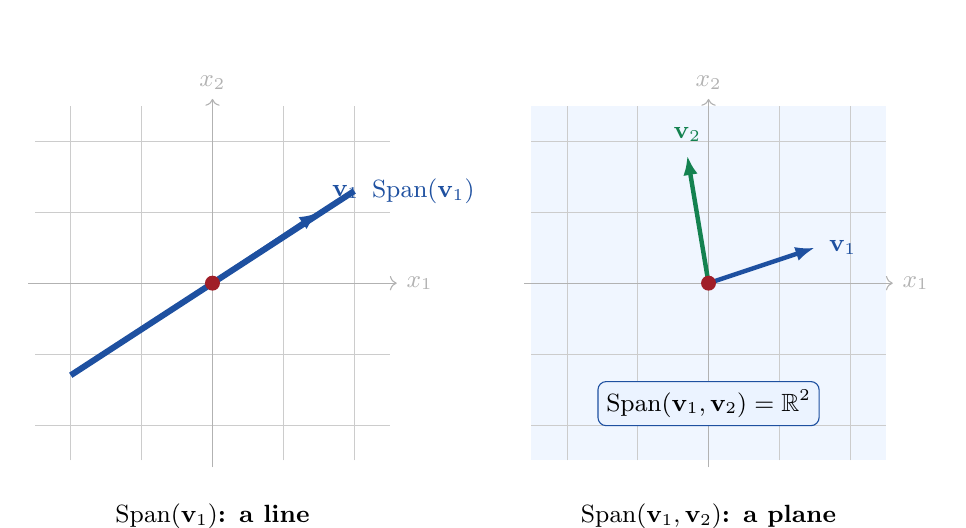
\begin{tikzpicture}[scale=0.9]
  %---- Span of one vector (a line) ------------------------------------------
  \begin{scope}
    \draw[gray!40, very thin] (-2.5,-2.5) grid (2.5,2.5);
    \draw[->,gray!60](-2.6,0)--(2.6,0)node[right]{\small$x_1$};
    \draw[->,gray!60](0,-2.6)--(0,2.6)node[above]{\small$x_2$};
    \draw[axiomblue, line width=2.2pt](-2.0,-1.3)--(2.0,1.3)
      node[right=2pt,font=\small]{$\Span(\vv{v}_1)$};
    \draw[-{Latex[length=7pt]}, axiomblue, line width=1.6pt]
      (0,0)--(1.5,1.0)node[above right=1pt,font=\small]{$\vv{v}_1$};
    \fill[thmred](0,0)circle(3pt);
    \node[font=\small\bfseries, below=2pt] at (0,-2.9)
      {$\Span(\vv{v}_1)$: a line};
  \end{scope}
  %---- Span of two non-parallel vectors (a plane) ---------------------------
  \begin{scope}[xshift=7cm]
    \fill[shadeblue!60](-2.5,-2.5)rectangle(2.5,2.5);
    \draw[gray!40, very thin](-2.5,-2.5)grid(2.5,2.5);
    \draw[->,gray!60](-2.6,0)--(2.6,0)node[right]{\small$x_1$};
    \draw[->,gray!60](0,-2.6)--(0,2.6)node[above]{\small$x_2$};
    \draw[-{Latex[length=7pt]}, axiomblue, line width=1.6pt]
      (0,0)--(1.5,0.5)node[right=1pt,font=\small]{$\vv{v}_1$};
    \draw[-{Latex[length=7pt]}, defgreen, line width=1.6pt]
      (0,0)--(-0.3,1.8)node[above=1pt,font=\small]{$\vv{v}_2$};
    \fill[thmred](0,0)circle(3pt);
    \node[draw=axiomblue,fill=shadeblue!80,rounded corners=3pt,
          font=\small,inner sep=3pt] at (0,-1.7)
      {$\Span(\vv{v}_1,\vv{v}_2)=\R^2$};
    \node[font=\small\bfseries, below=2pt] at (0,-2.9)
      {$\Span(\vv{v}_1,\vv{v}_2)$: a plane};
  \end{scope}
\end{tikzpicture}
\end{center}

% ══════════════════════════════════════════════════════════════════════════════
\section{Spanning Sets for a Vector Space}
% ══════════════════════════════════════════════════════════════════════════════

\begin{definition}{Spanning Set}{spanset}
  The set $\{\vv{v}_1, \ldots, \vv{v}_n\}$ is a \textbf{spanning set for $V$}
  if and only if every vector in $V$ can be written as a linear combination of
  $\vv{v}_1, \ldots, \vv{v}_n$; equivalently,
  \[
    \Span(\vv{v}_1, \ldots, \vv{v}_n) = V.
  \]
\end{definition}

\begin{example}{Standard spanning set for $\R^3$}{spanr3}
  Let
  \[
    \vv{e}_1 = \begin{pmatrix}1\\0\\0\end{pmatrix}, \quad
    \vv{e}_2 = \begin{pmatrix}0\\1\\0\end{pmatrix}, \quad
    \vv{e}_3 = \begin{pmatrix}0\\0\\1\end{pmatrix}.
  \]
  For any $(x_1, x_2, x_3)^T \in \R^3$:
  \[
    \begin{pmatrix}x_1\\x_2\\x_3\end{pmatrix}
    = x_1\vv{e}_1 + x_2\vv{e}_2 + x_3\vv{e}_3.
  \]
  Therefore $\{\vv{e}_1, \vv{e}_2, \vv{e}_3\}$ spans $\R^3$.
\end{example}

\begin{example}{Spanning set for $P_3$}{spanp3}
  The set $\{1,\, x,\, x^2\}$ spans $P_3$ because every polynomial of degree
  less than 3 can be written as:
  \[
    p(x) = a_0 \cdot 1 + a_1 \cdot x + a_2 \cdot x^2,
    \quad a_0, a_1, a_2 \in \R.
  \]
\end{example}

\noindent
The relationship between a vector space $V$, a spanning set, and the span is
illustrated below.

\begin{center}
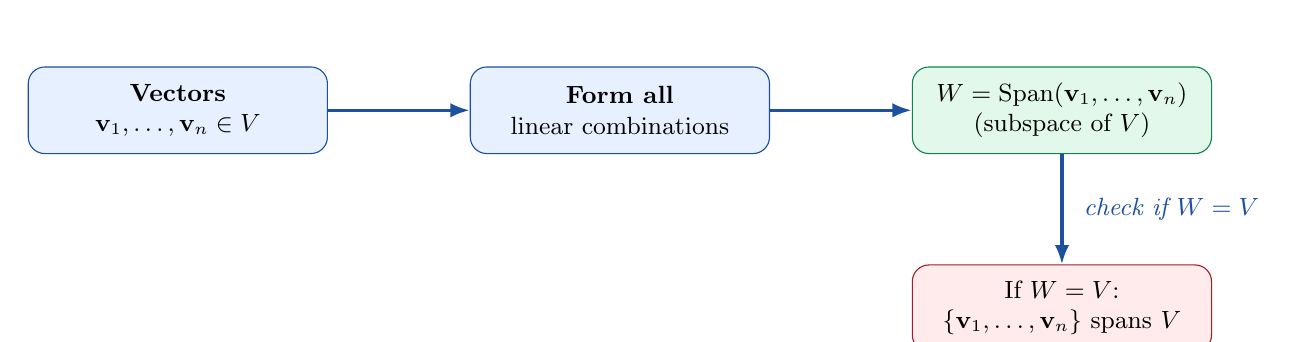
\begin{tikzpicture}[
  node distance=0.8cm,
  box/.style={draw=axiomblue, fill=shadeblue, rounded corners=6pt,
              minimum width=3.8cm, minimum height=1.1cm,
              align=center, font=\small},
  arr/.style={-{Latex[length=7pt]}, axiomblue, thick, line width=1.2pt}
]
  \node[box] (vs)   {\textbf{Vectors}\\$\vv{v}_1,\ldots,\vv{v}_n \in V$};
  \node[box, right=1.8cm of vs] (span)
    {\textbf{Form all}\\linear combinations};
  \node[draw=defgreen, fill=shadegreen, rounded corners=6pt,
        minimum width=3.8cm, minimum height=1.1cm,
        align=center, font=\small, right=1.8cm of span] (W)
    {$W = \Span(\vv{v}_1,\ldots,\vv{v}_n)$\\(subspace of $V$)};
  \node[draw=thmred, fill=shadered, rounded corners=6pt,
        minimum width=3.8cm, minimum height=1.1cm,
        align=center, font=\small, below=1.4cm of W] (full)
    {If $W = V$:\\$\{\vv{v}_1,\ldots,\vv{v}_n\}$ spans $V$};
  \draw[arr] (vs)   -- (span);
  \draw[arr] (span) -- (W);
  \draw[arr] (W)    -- (full) node[midway, right=4pt, font=\small\itshape]
    {check if $W=V$};
\end{tikzpicture}
\end{center}

% ══════════════════════════════════════════════════════════════════════════════
\section{Solution Structure of Linear Systems}
% ══════════════════════════════════════════════════════════════════════════════

\subsection{The Homogeneous Case: \texorpdfstring{$A\vv{x}=\vzero$}{Ax=0}}

When $\vv{b} = \vzero$, the solution set is $S = N(A)$, which — as proved in
Section~\ref{sec:nullspace} — is a subspace of $\R^n$.  In particular, it contains
$\vzero$, and any linear combination of solutions is again a solution.

\subsection{The Nonhomogeneous Case: \texorpdfstring{$A\vv{x}=\vv{b}$}{Ax=b} with
\texorpdfstring{$\vv{b}\neq\vzero$}{b ≠ 0}}

When $\vv{b} \neq \vzero$, the solution set is \emph{not} a subspace (it does not
contain $\vzero$ unless $\vzero$ is a solution, which would require $\vv{b}=\vzero$).
Nevertheless, it has a clean structure built from the null space.

\begin{theorem}{General Solution of a Consistent System (Theorem 3.2.2)}{thm322}
  Let $A\vv{x} = \vv{b}$ be a consistent $m\times n$ linear system and let
  $\vv{x}_0$ be a particular solution.  Then
  \[
    \boxed{
      \vv{y} \text{ is a solution to } A\vv{x}=\vv{b}
      \;\iff\;
      \vv{y} = \vv{x}_0 + \vv{z}, \quad \vv{z} \in N(A).
    }
  \]
  In other words, the complete solution set is
  \[
    S \;=\; \vv{x}_0 + N(A)
      \;=\; \bigl\{\, \vv{x}_0 + \vv{z} \;\big|\; \vv{z} \in N(A) \bigr\}.
  \]
\end{theorem}

\begin{proof}
\textbf{($\Leftarrow$)}\quad
Let $\vv{y} = \vv{x}_0 + \vv{z}$ with $\vv{z} \in N(A)$.  Then:
\[
  A\vv{y} = A(\vv{x}_0 + \vv{z}) = A\vv{x}_0 + A\vv{z} = \vv{b} + \vzero = \vv{b}.
\]

\textbf{($\Rightarrow$)}\quad
Let $\vv{y}$ be any solution, so $A\vv{y} = \vv{b}$.  Set $\vv{z} = \vv{y} - \vv{x}_0$.
Then:
\[
  A\vv{z} = A\vv{y} - A\vv{x}_0 = \vv{b} - \vv{b} = \vzero,
\]
so $\vv{z} \in N(A)$, giving $\vv{y} = \vv{x}_0 + \vv{z}$.
\end{proof}

\subsection{Geometric Interpretation}

\noindent
The solution set $S = \vv{x}_0 + N(A)$ is a \emph{translate} (or coset) of the
null space.  When $N(A)$ is a line through the origin in $\R^n$, the solution set
is a parallel line passing through $\vv{x}_0$.  When $N(A)$ is a plane, $S$ is a
parallel plane, and so on.

\begin{center}
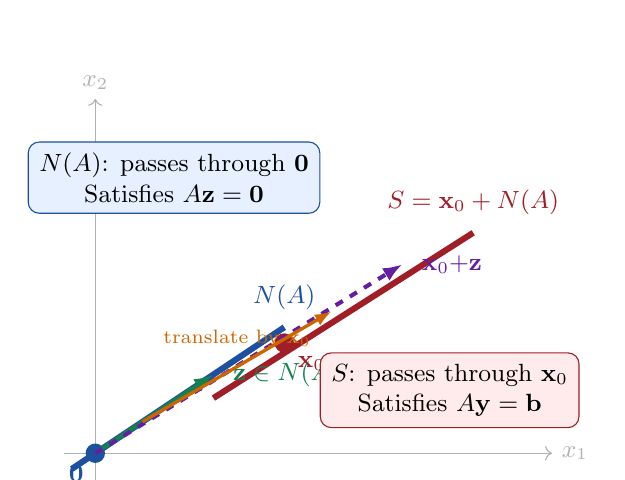
\begin{tikzpicture}[scale=1.0]
  %--- axes ---
  \draw[->,gray!60](-0.4,0)--(5.8,0)node[right]{\small$x_1$};
  \draw[->,gray!60](0,-0.4)--(0,4.5)node[above]{\small$x_2$};

  %--- N(A): a line through origin ---
  \draw[axiomblue, line width=2.2pt](-0.3,-0.2)--(2.4,1.6)
    node[above=2pt, axiomblue, font=\small]{$N(A)$};

  %--- x0 + N(A): the translated line ---
  \draw[thmred, line width=2.2pt](1.5,0.7)--(4.8,2.8)
    node[above=2pt, thmred, font=\small]{$S = \vv{x}_0+N(A)$};

  %--- x0 ---
  \fill[thmred](2.4,1.4)circle(3.5pt)
    node[below right=2pt, font=\small, thmred]{$\vv{x}_0$};

  %--- zero ---
  \fill[axiomblue](0,0)circle(3.5pt)
    node[below left=1pt, font=\small, axiomblue]{$\vzero$};

  %--- z vector ---
  \draw[-{Latex[length=7pt]}, defgreen, line width=1.5pt]
    (0,0)--(1.5,1.0)
    node[right=3pt, font=\small, defgreen]{$\vv{z}\in N(A)$};

  %--- x0 + z ---
  \draw[-{Latex[length=7pt]}, purpledark, line width=1.5pt, dashed]
    (0,0)--(3.9,2.4)
    node[right=3pt, font=\small, purpledark]{$\vv{x}_0{+}\vv{z}$};

  %--- parallel arrows showing translation ---
  \draw[-{Latex[length=6pt]}, orange!80!black, line width=1.2pt]
    (0.6,0.4)--(3.0,1.8)
    node[midway, above=3pt, font=\scriptsize, orange!80!black]
    {translate by $\vv{x}_0$};

  %--- annotations ---
  \node[draw=axiomblue, fill=shadeblue, rounded corners=4pt,
        font=\small, align=center, inner sep=4pt] at (1.0,3.5)
    {$N(A)$: passes through $\vzero$\\
     Satisfies $A\vv{z}=\vzero$};
  \node[draw=thmred, fill=shadered, rounded corners=4pt,
        font=\small, align=center, inner sep=4pt] at (4.5,0.8)
    {$S$: passes through $\vv{x}_0$\\
     Satisfies $A\vv{y}=\vv{b}$};
\end{tikzpicture}
\end{center}

\subsection{Worked Example}

\begin{example}{Complete solution of $A\vv{x}=\vv{b}$}{solnex}
  Let
  \[
    A = \begin{pmatrix}1 & 2 & 1\\2 & 4 & 3\end{pmatrix},
    \quad
    \vv{b} = \begin{pmatrix}3\\8\end{pmatrix}.
  \]

  \textbf{Step 1: Find a particular solution.}\quad
  Row-reduce $[A\mid\vv{b}]$:
  \[
    \begin{pmatrix}1&2&1&3\\2&4&3&8\end{pmatrix}
    \xrightarrow{R_2-2R_1}
    \begin{pmatrix}1&2&1&3\\0&0&1&2\end{pmatrix}
    \xrightarrow{R_1-R_2}
    \begin{pmatrix}1&2&0&1\\0&0&1&2\end{pmatrix}.
  \]
  Setting the free variable $x_2 = 0$: $x_1 = 1,\; x_3 = 2$.
  A particular solution is $\vv{x}_0 = (1,\, 0,\, 2)^T$.

  \textbf{Step 2: Find $N(A)$.}\quad
  With $x_2 = s$ free and $\vv{b}=\vzero$: $x_1=-2s,\; x_3=0$.
  \[
    N(A) = \Span\!\left(\begin{pmatrix}-2\\1\\0\end{pmatrix}\right).
  \]

  \textbf{Step 3: Write the complete solution.}
  \[
    \vv{x}
    = \vv{x}_0 + \vv{z}
    = \begin{pmatrix}1\\0\\2\end{pmatrix}
    + s\begin{pmatrix}-2\\1\\0\end{pmatrix},
    \quad s \in \R.
  \]
\end{example}

% ══════════════════════════════════════════════════════════════════════════════
\section{Summary and Connections}
% ══════════════════════════════════════════════════════════════════════════════

\begin{tcolorbox}[
  enhanced, colback=shadeyellow, colframe=orange!70!black,
  title={\bfseries Chapter Summary}, breakable
]
\begin{itemize}[leftmargin=1.5em, itemsep=0.5em]
  \item A \textbf{subspace} $S$ of a vector space $V$ is a nonempty subset closed
        under scalar multiplication and addition; it is itself a vector space.
  \item Every subspace contains $\vzero$; use this to check nonemptiness.
  \item The \textbf{trivial subspaces} of $V$ are $\{\vzero\}$ and $V$ itself.
  \item The \textbf{null space} $N(A) = \{\vv{x}\in\R^n \mid A\vv{x}=\vzero\}$ is
        always a subspace of $\R^n$.
  \item A \textbf{linear combination} of vectors $\vv{v}_1,\ldots,\vv{v}_n$ is any
        sum $\alpha_1\vv{v}_1+\cdots+\alpha_n\vv{v}_n$.
  \item The \textbf{span} of a set of vectors is the set of all their linear
        combinations; it is always a subspace.
  \item $\{\vv{v}_1,\ldots,\vv{v}_n\}$ is a \textbf{spanning set} for $V$ when
        every vector in $V$ is a linear combination of them.
  \item For a consistent system $A\vv{x}=\vv{b}$, the general solution is
        $\vv{y} = \vv{x}_0 + \vv{z}$, where $\vv{x}_0$ is any particular
        solution and $\vv{z}$ ranges over $N(A)$.
\end{itemize}
\end{tcolorbox}

\medskip
\noindent
The following diagram summarises all the key relationships covered in this chapter.

\begin{center}
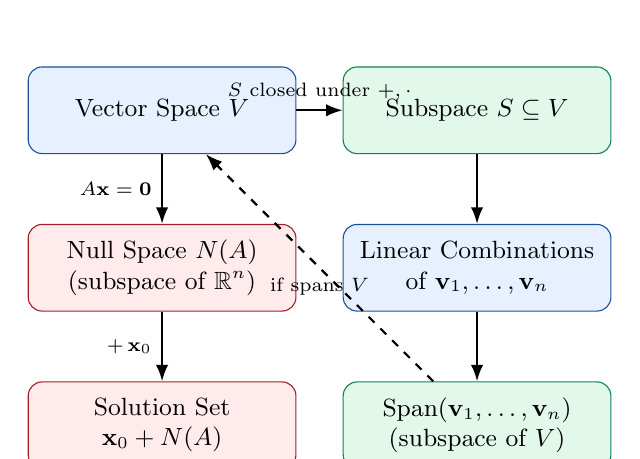
\begin{tikzpicture}[
  every node/.style={font=\small},
  cbox/.style={draw=axiomblue, fill=shadeblue, rounded corners=5pt,
               minimum width=3.4cm, minimum height=1.1cm, align=center},
  gbox/.style={draw=defgreen, fill=shadegreen, rounded corners=5pt,
               minimum width=3.4cm, minimum height=1.1cm, align=center},
  rbox/.style={draw=thmred, fill=shadered, rounded corners=5pt,
               minimum width=3.4cm, minimum height=1.1cm, align=center},
  arr/.style={-{Latex[length=6pt]}, thick}
]
  \node[cbox] (V)  at (0,0)    {Vector Space $V$};
  \node[gbox] (S)  at (4,0)    {Subspace $S\subseteq V$};
  \node[cbox] (lc) at (4,-2)   {Linear Combinations\\of $\vv{v}_1,\ldots,\vv{v}_n$};
  \node[gbox] (sp) at (4,-4)   {$\Span(\vv{v}_1,\ldots,\vv{v}_n)$\\(subspace of $V$)};
  \node[rbox] (NA) at (0,-2)   {Null Space $N(A)$\\(subspace of $\R^n$)};
  \node[rbox] (sol)at (0,-4)   {Solution Set\\$\vv{x}_0 + N(A)$};

  \draw[arr] (V)  -- node[above, font=\scriptsize]{$S$ closed under $+,\cdot$} (S);
  \draw[arr] (S)  -- (lc);
  \draw[arr] (lc) -- (sp);
  \draw[arr] (V)  -- node[left, font=\scriptsize]{$A\vv{x}=\vzero$} (NA);
  \draw[arr] (NA) -- node[left, font=\scriptsize]{$+\,\vv{x}_0$} (sol);
  \draw[arr, dashed] (sp) -- node[below, font=\scriptsize]{if spans $V$} (V);
\end{tikzpicture}
\end{center}

% ══════════════════════════════════════════════════════════════════════════════
\end{document}
% ══════════════════════════════════════════════════════════════════════════════
